\documentclass[10pt]{article}
\usepackage[polish]{babel}
\usepackage[utf8]{inputenc}
\usepackage[T1]{fontenc}
\usepackage{amsmath}
\usepackage{amsfonts}
\usepackage{amssymb}
\usepackage[version=4]{mhchem}
\usepackage{stmaryrd}
\usepackage{graphicx}
\usepackage[export]{adjustbox}
\graphicspath{ {./images/} }

\title{I Konkurs matematyczny St@s \\
 XIV LO im. Stanisława Staszica 29 maja 2001 roku }

\author{}
\date{}


\begin{document}
\maketitle
\section*{klasa VI}
Na rozwiqzanie poniżsych zadań masz 90 minut. Kolejność rozwiqzywania rych zadañ jest dowolna.\\
\(W_{\text {szystkie zadania sq jednakowo punktowane. Maksymalnq liczbę punktów może uzyskać jedynie }}\) pelne rozwiqzanie, z uzasadnieniem i odpowiedziq.\\
Używanie korektora i korzystanie z kalkulatora jest niedozwolone.

\section*{Zadanie 1.}
Takim samym literom odpowiadają takie same cyfry, a różnym literom - różne cyfry. Znajdż te cyfry, tak aby wszystkie działania w pionie i wszystkie działania w poziomie były prawdziwe.

\begin{center}
\begin{tabular}{cc}
\(\mathrm{AA}+\mathrm{BCD}=\mathrm{ECF}\) &  \\
\(+\quad+\) & + \\
\(\mathrm{B}+\mathrm{DD}\) & \(=\mathrm{DH}\) \\
\hline
\(\mathrm{BCC}+\mathrm{BHC}\) & \(=\mathrm{EHC}\) \\
\hline
\end{tabular}
\end{center}

\section*{Zadanie 2.}
Czy jest taka pięciocyfrowa liczba pierwsza, którą można zapisać używajạc jednokrotnie każdej z cyfr: 2, 3, 4, 7, 8? Odpowiedż uzasadnij.

\section*{Zadanie 3.}
Trzynaście osób ma usiąść wokỏł okrąglego stołu. Każda z nich ma inną liczbę monet. Uzasadnij, że niezależnie od tego, gdzie kto usiądzie, zawsze będzie można znaleźć takie dwie sąsiednie osoby, które w sumie będą miały parzystą liczbę monet.

\section*{Zadanie 4.}
Dwa boki pewnego trójkąta są równe i każdy z nich ma 6 cm . Pole tego trójkąta jest równe \(18 \mathrm{~cm}^{2}\). Znajdź kąty tego trójkąta. Odpowiedź uzasadnij.

\section*{Zadanie 5.}
Na trzech ṡcianach sześcianu narysowano symbole. Przerysuj siatkę tego sześcianu i dorysuj na niej brakujące elementy.\\
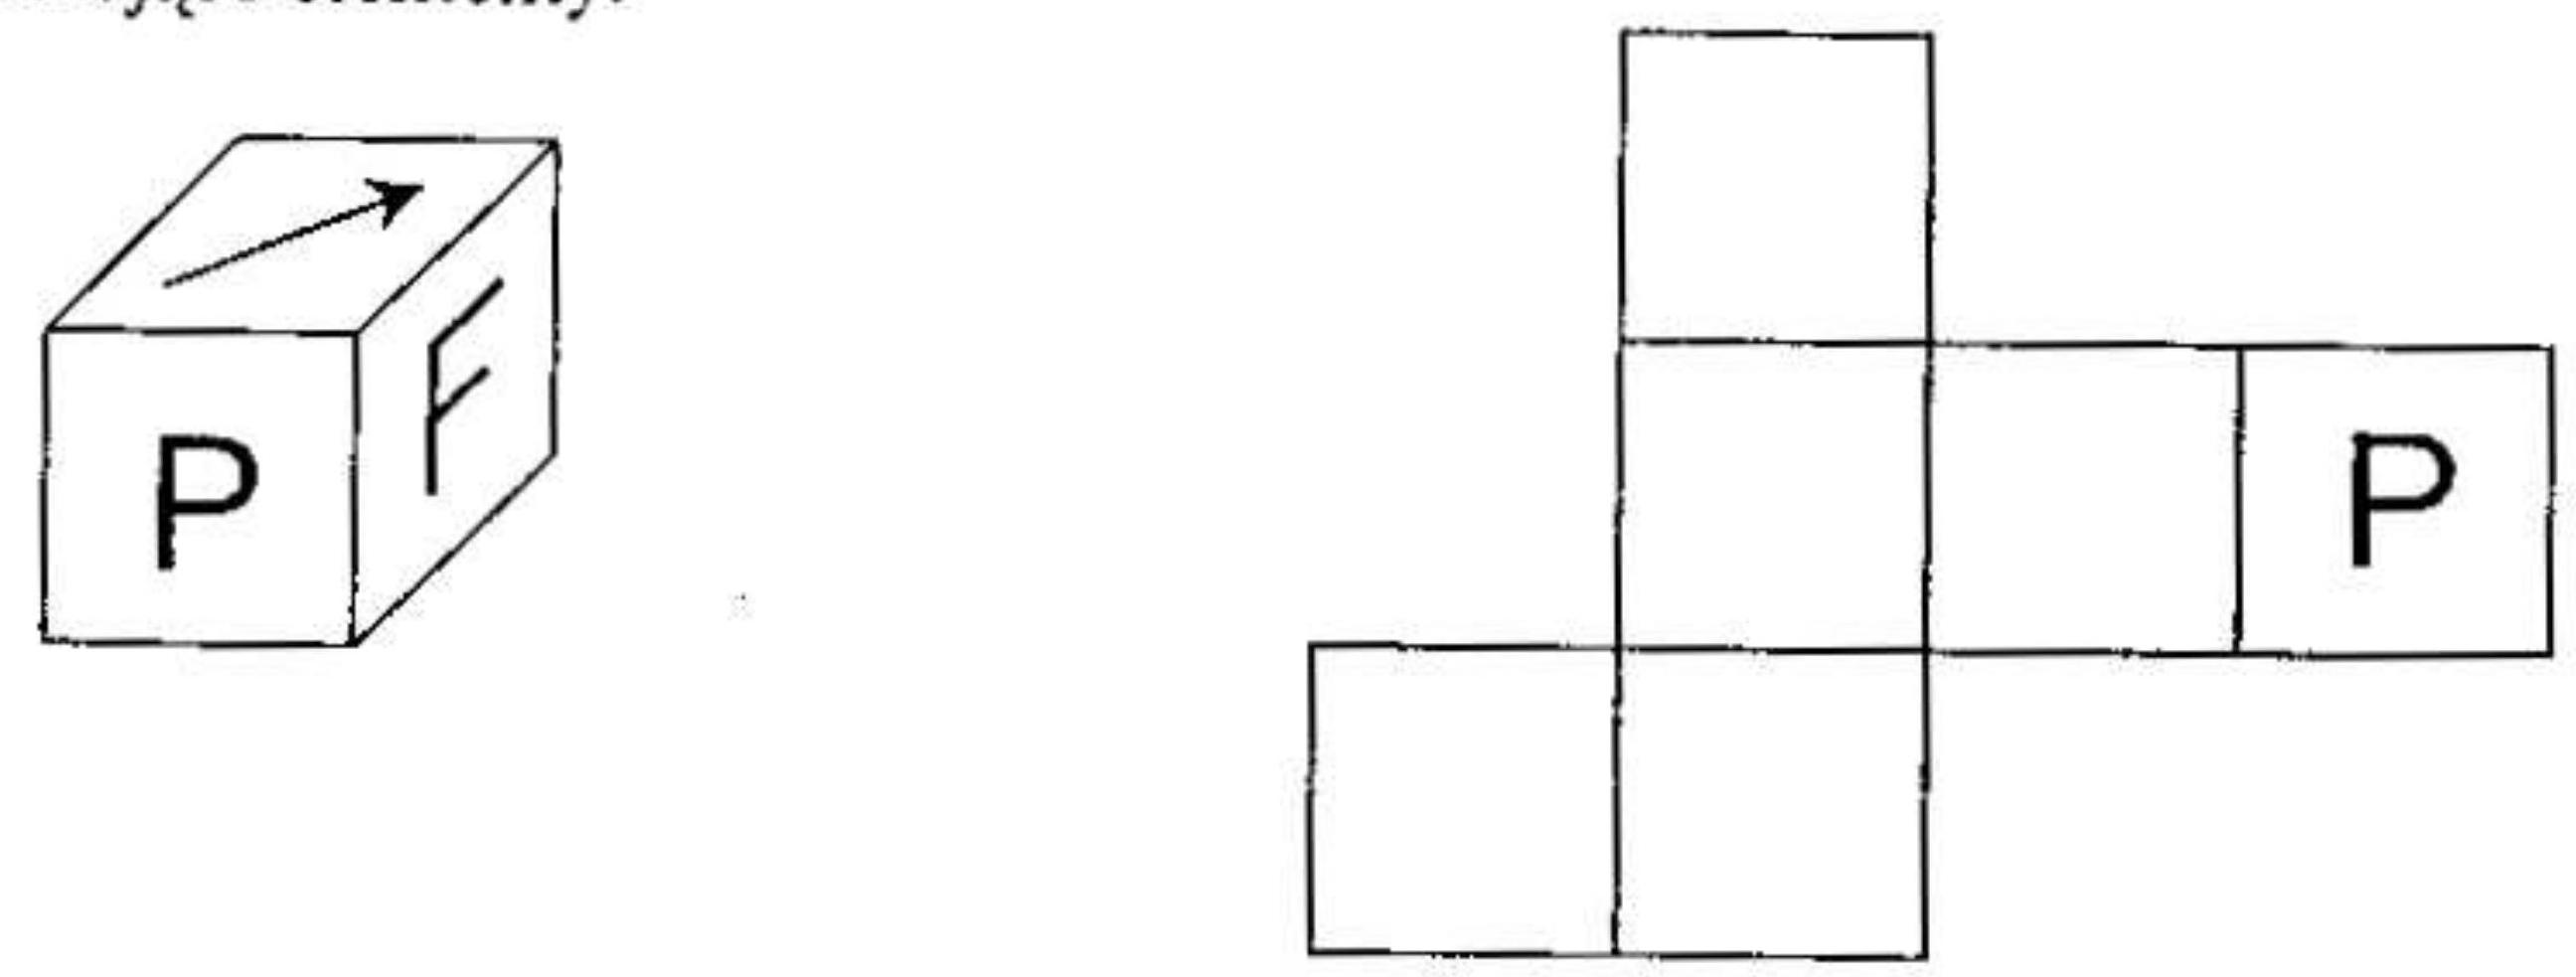
\includegraphics[max width=\textwidth, center]{2024_11_21_1724fd187094cf40e180g-1}


\end{document}